%%%%%%%%%%%%%%%%%%%%%%%%%%%%%%%%%%%%%%%%%
% a0poster Landscape Poster
% LaTeX Template
% Version 1.0 (22/06/13)
%
% The a0poster class was created by:
% Gerlinde Kettl and Matthias Weiser (tex@kettl.de)
% 
% This template has been downloaded from:
% http://www.LaTeXTemplates.com
%
% License:
% CC BY-NC-SA 3.0 (http://creativecommons.org/licenses/by-nc-sa/3.0/)
%
%%%%%%%%%%%%%%%%%%%%%%%%%%%%%%%%%%%%%%%%%

%----------------------------------------------------------------------------------------
%	PACKAGES AND OTHER DOCUMENT CONFIGURATIONS
%----------------------------------------------------------------------------------------

\documentclass[a0,landscape]{a0poster}
\setlength{\topmargin}{-1in}
 \setlength{\paperheight}{30.0in} % A0 height: 33.1in

\usepackage{multicol} % This is so we can have multiple columns of text side-by-side 
\columnsep=30pt % This is the amount of white space between the columns in the poster 
\columnseprule=0pt % This is the thickness of the black line between the columns in the poster

\usepackage[svgnames]{xcolor} % Specify colors by their 'svgnames',
                              % for a full list of all colors
                              % available see here: http://www.latextemplates.com/svgnames-colors

\usepackage{times} % Use the times font
%\usepackage{palatino} % Uncomment to use the Palatino font

\usepackage{graphicx} % Required for including images
\graphicspath{{figures/}} % Location of the graphics files
\usepackage{booktabs} % Top and bottom rules for table
\usepackage[font=small,labelfont=bf]{caption} % Required for specifying captions to tables and figures 
\usepackage{amsfonts,
  amsmath, amsthm, amssymb} % For math fonts, symbols and environments
\usepackage{wrapfig} % Allows wrapping text around tables and figures

\usepackage{Sweave}
\begin{document}
\Sconcordance{concordance:conference_poster_5.tex:/Users/hermes/projects/esa2015/poster_2015/docs/poster/conference_poster_5.Rnw:%
1 43 1 1 0 197 1 1 8 1 3 5 1 1 13 1 3 4 1 1 46 1 3 59 1}


%----------------------------------------------------------------------------------------
%	POSTER HEADER 
%----------------------------------------------------------------------------------------

% The header is divided into three boxes:
% The first is 55% wide and houses the title, subtitle, names and university/organization
% The second is 25% wide and houses contact information
% The third is 19% wide and houses a logo for your university/organization or a photo of you
% The widths of these boxes can be easily edited to accommodate your content as you see fit

\begin{minipage}[b]{0.65\linewidth}
\veryHuge \color{Red} \textbf{Temporal scales of coupled ecosystem
  processes provide a benchmark for alternate ecosystem states}
\color{Black}\\ % Title 
\Huge\textit{Photosynthesis and decomposition in a model micro-ecosystem}\\[1cm] % Subtitle 
\huge \textbf{Matthew K. Lau \& Aaron M. Ellison}\\ % Author(s) 
\huge Harvard Forest, Harvard University \\ % University/organization
\end{minipage}
%
\begin{minipage}[b]{0.20\linewidth}
\color{DarkSlateGray}\Large \textbf{Contact Information:}\\ 
Harvard Forest\\ % Address 
Harvard University\\ 324 N Main St, Petersham, MA, USA\\ 
Phone: +1 (978) 756-6165\\ % Phone number 
Email: \texttt{matthewklau@fas.harvard.edu}\\ % Email address
\end{minipage}
%
\begin{minipage}[t]{0.12\linewidth}

\includegraphics[width=17cm]{hf.pdf} % Logo or a photo of you, adjust its dimensions here
%% 
\includegraphics[width=10cm]{harvard.png} % Logo or a photo of you, adjust its dimensions here
\end{minipage}

\vspace{1cm} % A bit of extra whitespace between the header and poster
             % content

%----------------------------------------------------------------------------------------

\begin{multicols}{4} % This is how many columns your poster will be broken into, a poster with many figures may benefit from less columns whereas a text-heavy poster benefits from more

%----------------------------------------------------------------------------------------
%	ABSTRACT
%----------------------------------------------------------------------------------------

\color{DarkBlue} % Navy color for the abstract

\section*{Summary}
  
  \begin{itemize}
  \item Community dynamics can lead to sudden, recalcitrant ecosystem
    state changes (aka. tipping points),
  \item Here, we further develop and apply the micro-ecosystem model
    based on the food web of the carnivorous plant, \textit{Sarracenia
      purpurea}, to simulate oxygen production of how perturbations
    lead to ecosystem state changes,
  \item We found three main results:
    \begin{enumerate}
    \item The micro-ecosystem model reproduced the gross behavior of
      the pitcher plant food web
    \item Sensitivity analysis revealed parameter combinations that
      produce alternative ecosystem states
    \item Differences in photosynthesis and decomposition rates lead
      to both alternative states and hyesteresis,
    \end{enumerate}
  \item These results point to a general framework for identifying
    potential ecosystem state changes. 
  \end{itemize}

%----------------------------------------------------------------------------------------
%	INTRODUCTION
%----------------------------------------------------------------------------------------

% \color{SaddleBrown} % SaddleBrown color for the introduction

%% \section*{Background}

%% \begin{itemize}
%% \item Stability
%% \item Alternative states
%% \item Tipping points
%% \item The pitcher plant micro-ecosystem
%% \item Hastings, temporal scales paper
%% \end{itemize}

%----------------------------------------------------------------------------------------
%	OBJECTIVES
%----------------------------------------------------------------------------------------

\color{DarkSlateGray} % DarkSlateGray color for the rest of the content

%% \section*{Hypotheses}


%----------------------------------------------------------------------------------------
%	MATERIALS AND METHODS
%----------------------------------------------------------------------------------------

\section*{Methods}

%------------------------------------------------

\subsection*{The pitcher plant micro-ecosystem}

\begin{itemize}
\item History of research (Darwin to Sirota)
\item Ideal for studying food-web dynamics
\end{itemize}

\begin{center}\vspace{1cm}
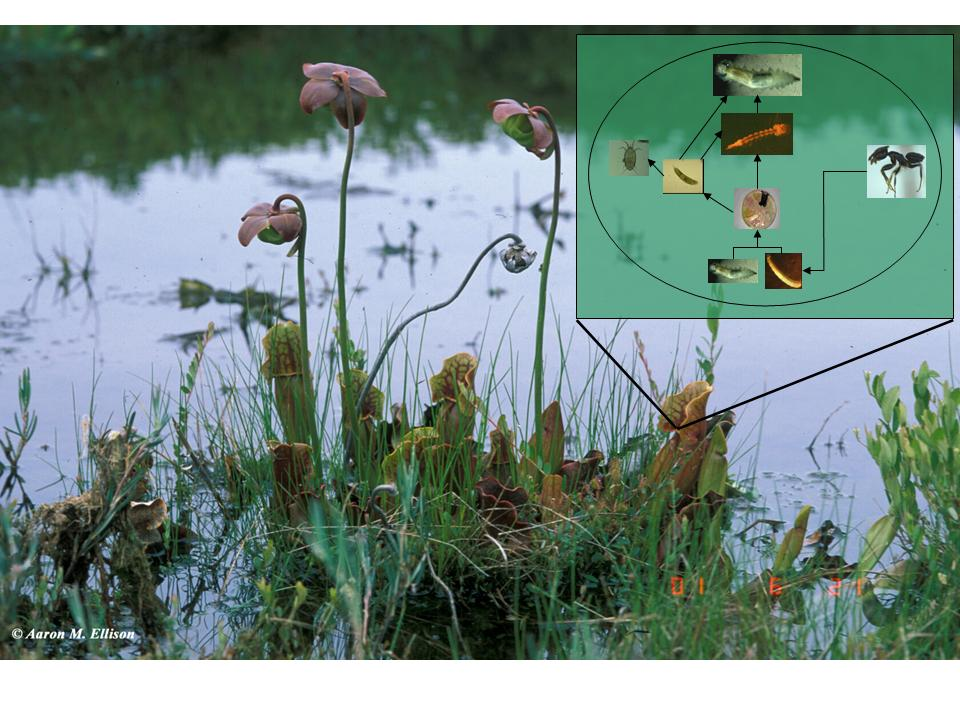
\includegraphics[width=0.95\linewidth]{spfoodweb}
\captionof{figure}{\color{Green} Pitcher plant and food web.}
\end{center}\vspace{1cm}

\subsection*{The model and simulations}

The general model for alternative stable states:

\begin{equation}
\frac{dx}{dt} = a - bx + r f(x)
\label{eqn:carpenter}
\end{equation}


\begin{itemize}
\item $x$ = observed variable
\item $a$ = positively correlated state variable
\item $b$ = negatively correlated state variable
\item $rf(x)$ = positive feedback loop, where $r$ controls the rate
  and $f(x)$ determines the shape of the state transition
\end{itemize}

The pitcher plant micro-ecosystem model:

\begin{equation}
x_{t+1} = a_t A_t - \left\{m + a_t \frac{w+t}{K + w_t}\right\} +
D_t(x_t)
\label{eqn:ppme}
\end{equation}



\begin{equation}
  A = A_{max} \left\{ 1 - e^{-0.3 (PAR - LCP)} \right\} 
  \label{eqn:photosynthesis}
\end{equation}

\begin{equation}
PAR = c \sin(2 \pi f)
\label{eqn:PAR}
\end{equation}

\begin{equation}
w_t = e^{-\beta w_0 t}
\label{eqn:decomp}
\end{equation}

\begin{equation}
a_t+1 = a_t \left\{ \frac{a'_{max}-a'_{min}}{1+e^{-s n_t - d}} + a'_{min}\right\}
\label{eqn:oxygenation}
\end{equation}

\begin{equation}
n_t = \frac{w_t x_t}{c}
\label{eqn:nutrients}
\end{equation}


%% $R^2 = $ 0.1092

%% \begin{center}\vspace{1cm}
%% \begin{tabular}{l l l l}
%% \toprule
%% \textbf{Parameter} & \textbf{Min} & \textbf{Max} \\
%% \midrule
%% $w$ (prey mass) & 0 & 10 \\
%% $\beta$ (decomp rate) & 0.001 & 0.011 \\
%% $d$ (inflection point) & -5 & 5 \\
%% \bottomrule
%% \end{tabular}
%% \captionof{table}{\color{Green} Parameter ranges for simulations.}
%% \end{center}\vspace{1cm}





%----------------------------------------------------------------------------------------
%	RESULTS 
%----------------------------------------------------------------------------------------

\section*{Results}
The model reproduces the basic features of the pitcher plant system:

\begin{itemize}
\item Photosynthesis oscillates daily.
\item Decomposition takes 48 hours to complete.
\item Hysteresis occurrs when the system is loaded with prey. 
\end{itemize}


\begin{block}{}
\setkeys{Gin}{width=0.90\linewidth}

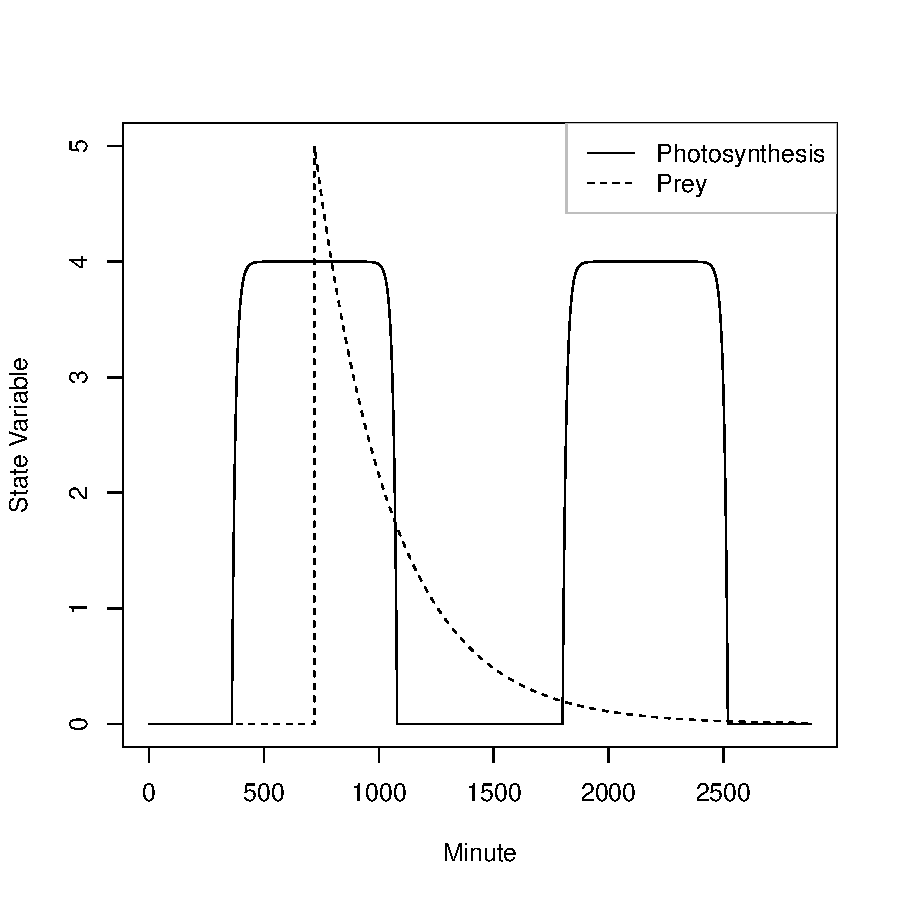
\includegraphics{conference_poster_5-base}

\end{block}


\begin{block}{}
\setkeys{Gin}{width=0.9\linewidth}
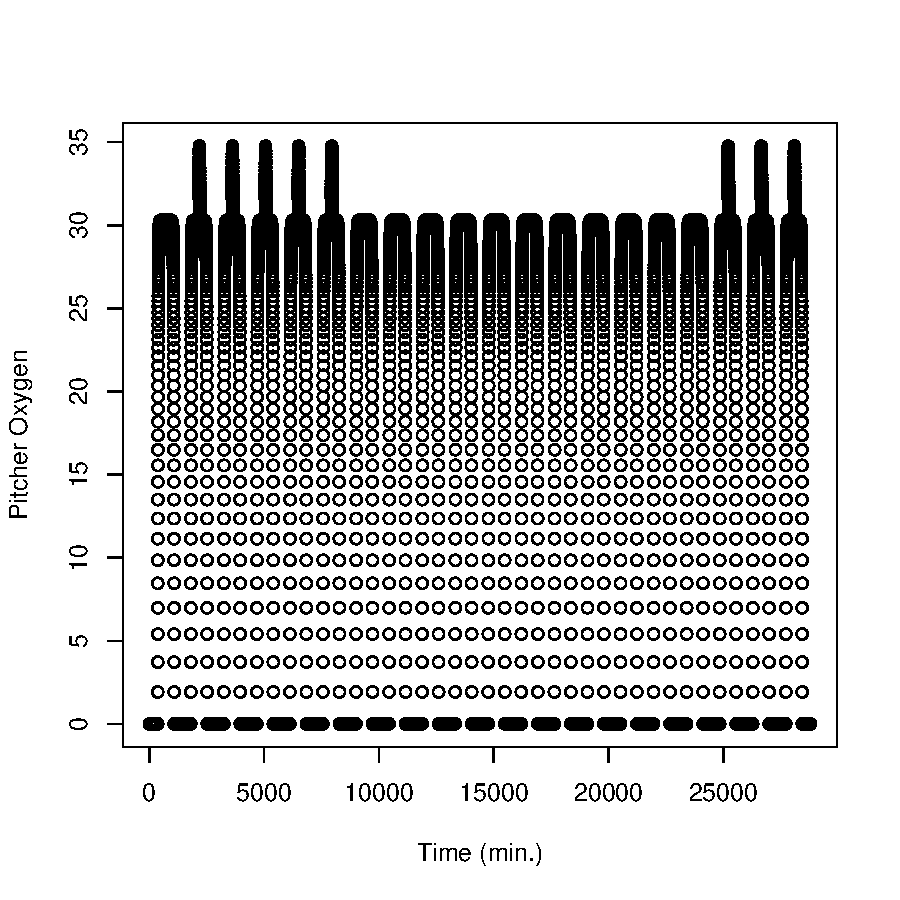
\includegraphics{conference_poster_5-hyst}

\end{block}

\begin{block}
\setkeys{Gin}{width=0.7\linewidth}  
\includegraphics{conference_poster_5-sens}

\end{block}

%----------------------------------------------------------------------------------------
%	CONCLUSIONS
%----------------------------------------------------------------------------------------

\color{SaddleBrown} % SaddleBrown color for the conclusions to make them stand out

\section*{Conclusions}

\begin{itemize}
\item Exploration of the parameter space for the model supports the
  presence of alternative states and the potential for tipping points
  resulting from the impact of the rate of decomposition and
  photosynthesitic augmentation.
\item These results suggest that identifying the flow of important
  components (e.g., nutrients) among compartments in ecosystems and
  using snap-shot data to compare the temporal scale of these flow
  rates can help to detect systems prone to critical transitions.
\item We are currently developing a toolbox for exploring ecosystems
  models using a web-based dynamic modeling framework available at:
  https://github.com/HarvardForest/ecoapps.
\end{itemize}

\color{DarkSlateGray} % Set the color back to DarkSlateGray for the rest of the content

%----------------------------------------------------------------------------------------
%	FORTHCOMING RESEARCH
%----------------------------------------------------------------------------------------

%% \section*{Forthcoming}


%----------------------------------------------------------------------------------------
%	REFERENCES
%----------------------------------------------------------------------------------------

\nocite{*} % Print all references regardless of whether they were cited in the poster or not
\bibliographystyle{plain} % Plain referencing style
\bibliography{sample} % Use the example bibliography file sample.bib

%----------------------------------------------------------------------------------------
%	ACKNOWLEDGEMENTS
%----------------------------------------------------------------------------------------

\section*{Acknowledgements}

Thanks are owed to a number of collaborators, including B. Baiser
(UFL), N. Gotelli (UVM) and A. Northrop (UVM). Funding was provided by
NSF Grant (XXX-XXXX). 

%----------------------------------------------------------------------------------------

\end{multicols}
\end{document}
